\chapter{Cadre du Projet, Gouvernance et Analyse du Besoin}

\section{Présentation de l'Organisme d'Accueil}
Le présent projet s'inscrit dans le cadre d'une étude analytique au sein de l'École Nationale de l'Intelligence Artificielle et du Digital (ENIAD). L'objectif est de simuler une intervention de conseil en Business Intelligence pour une entreprise de services moderne faisant face à des défis de gestion de son capital humain. L'organisation cible, bien que fictive pour les besoins de l'exercice, reflète les enjeux réels des départements RH actuels : besoin de réactivité, optimisation de la rétention et pilotage par la performance.

\section{Étude de l'Existant et Critique}
Actuellement, l'entreprise gère ses données RH de manière fragmentée. Les informations sont extraites de divers systèmes (ERP, fichiers de pointage) et consolidées manuellement sous forme de classeurs Excel isolés.

\subsection{Limites identifiées}
\begin{itemize}
    \item \textbf{Processus chronophages :} La collecte et le nettoyage manuel des données occupent plus de 60\% du temps des analystes RH.
    \item \textbf{Risques d'erreurs :} Les manipulations manuelles (copier-coller, formules Excel complexes) entraînent des incohérences dans les rapports finaux.
    \item \textbf{Manque de flexibilité :} Les rapports sont statiques. Toute nouvelle demande d'analyse nécessite une refonte complète du fichier.
    \item \textbf{Absence de source unique :} Il n'existe pas de référentiel centralisé, ce qui conduit à des chiffres divergents entre les départements.
\end{itemize}

\begin{figure}[h]
    \centering
    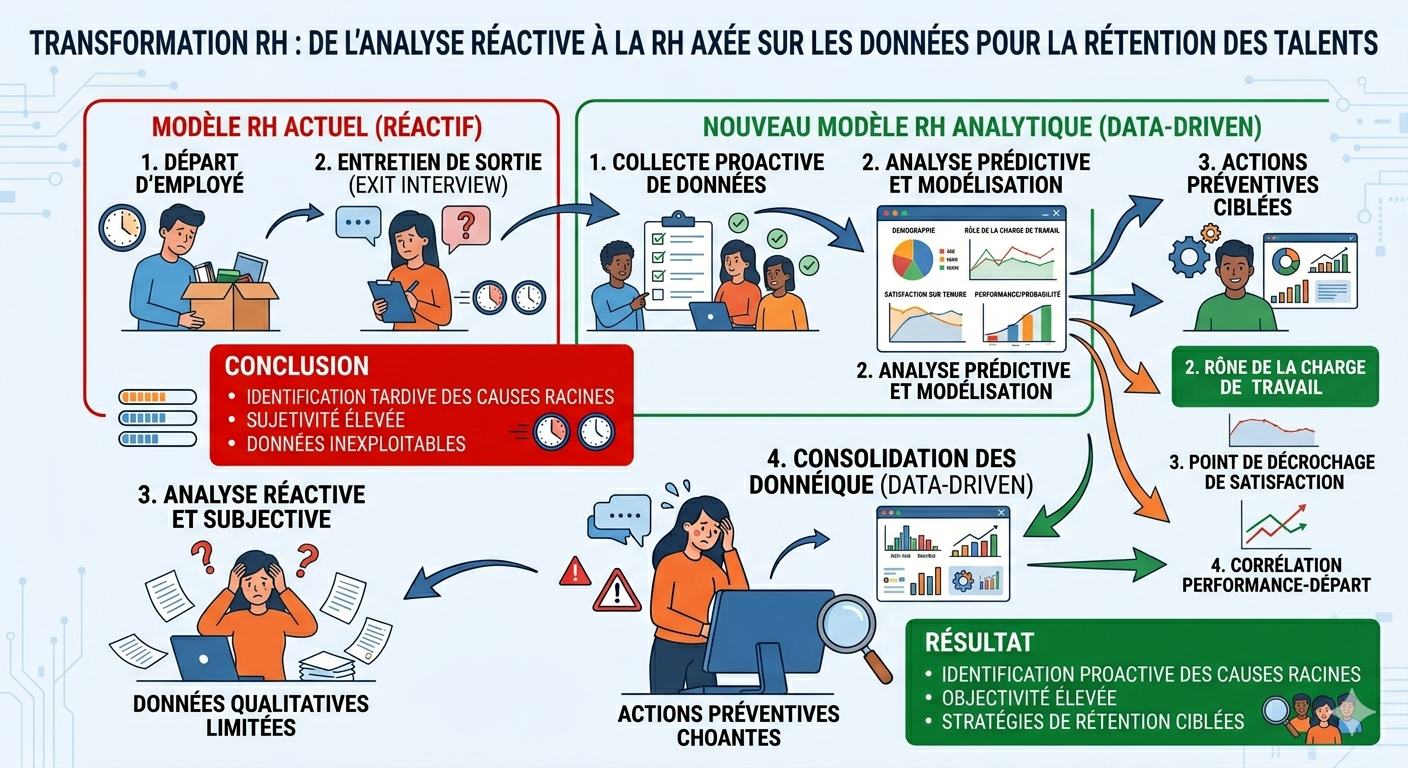
\includegraphics[width=0.8\textwidth]{figures/fig1_1_existant.png}
    \caption{Schéma de la circulation de l'information existante}
    \label{fig:existant}
\end{figure}

\section{Spécification des Besoins}

\subsection{Besoins fonctionnels}
\begin{itemize}
    \item \textbf{Calcul automatisé du Headcount :} Suivi en temps réel de l'effectif total et actif.
    \item \textbf{Analyse de l'Attrition :} Calcul dynamique du taux de départ et identification des segments à risque.
    \item \textbf{Suivi de la Satisfaction :} Corrélation entre le climat social et la rétention.
    \item \textbf{Pilotage de la Masse Salariale :} Vision globale des rémunérations par département et job role.
    \item \textbf{Filtrage dynamique :} Capacité de segmenter tous les indicateurs par période, département et genre.
\end{itemize}

\subsection{Besoins non-fonctionnels}
\begin{itemize}
    \item \textbf{Performance :} Temps de réponse des visuels inférieur à 2 secondes malgré le volume de données.
    \item \textbf{Ergonomie :} Interface intuitive respectant les codes du Data Storytelling (Thème Executive 3D).
    \item \textbf{Maintenabilité :} Architecture modulaire permettant d'ajouter de nouvelles sources facilement.
\end{itemize}

\section{Organisation de l'Équipe et Méthodologie}

Pour garantir le succès du projet, nous avons adopté une organisation par rôles spécialisés, s'appuyant sur un workflow Git rigoureux :

\begin{itemize}
    \item \textbf{Zakariae EL HADDOUCHI (Data Engineer) :} Responsable du pipeline ETL (\textit{branch: feature/etl-pipeline}). En charge de la connexion, du nettoyage et de la structuration des flux bruts.
    \item \textbf{Oussama LEBYED (Data Architect) :} Responsable de la modélisation dimensionnelle (\textit{branch: feature/data-modeling}). En charge du Schéma en Étoile et de l'intégrité des relations.
    \item \textbf{Meryame EL AIBOUDI (Business Analyst) :} Responsable de la logique analytique et documentation (\textit{branch: feature/kpi-logic}). En charge des mesures DAX et du dictionnaire de données.
    \item \textbf{Oualid BOUTAYEB (Data Visualizer) :} Responsable du design et du storytelling (\textit{branch: feature/dashboard-design}). En charge de l'UI/UX et de la restitution graphique.
\end{itemize}

\section{Planification et Suivi}
Le projet a été découpé en lots de travail suivant une approche agile. Le suivi a été assuré par un diagramme de Gantt permettant de visualiser les dépendances entre les phases ETL, Modélisation et Visualisation.

\begin{figure}[h]
    \centering
    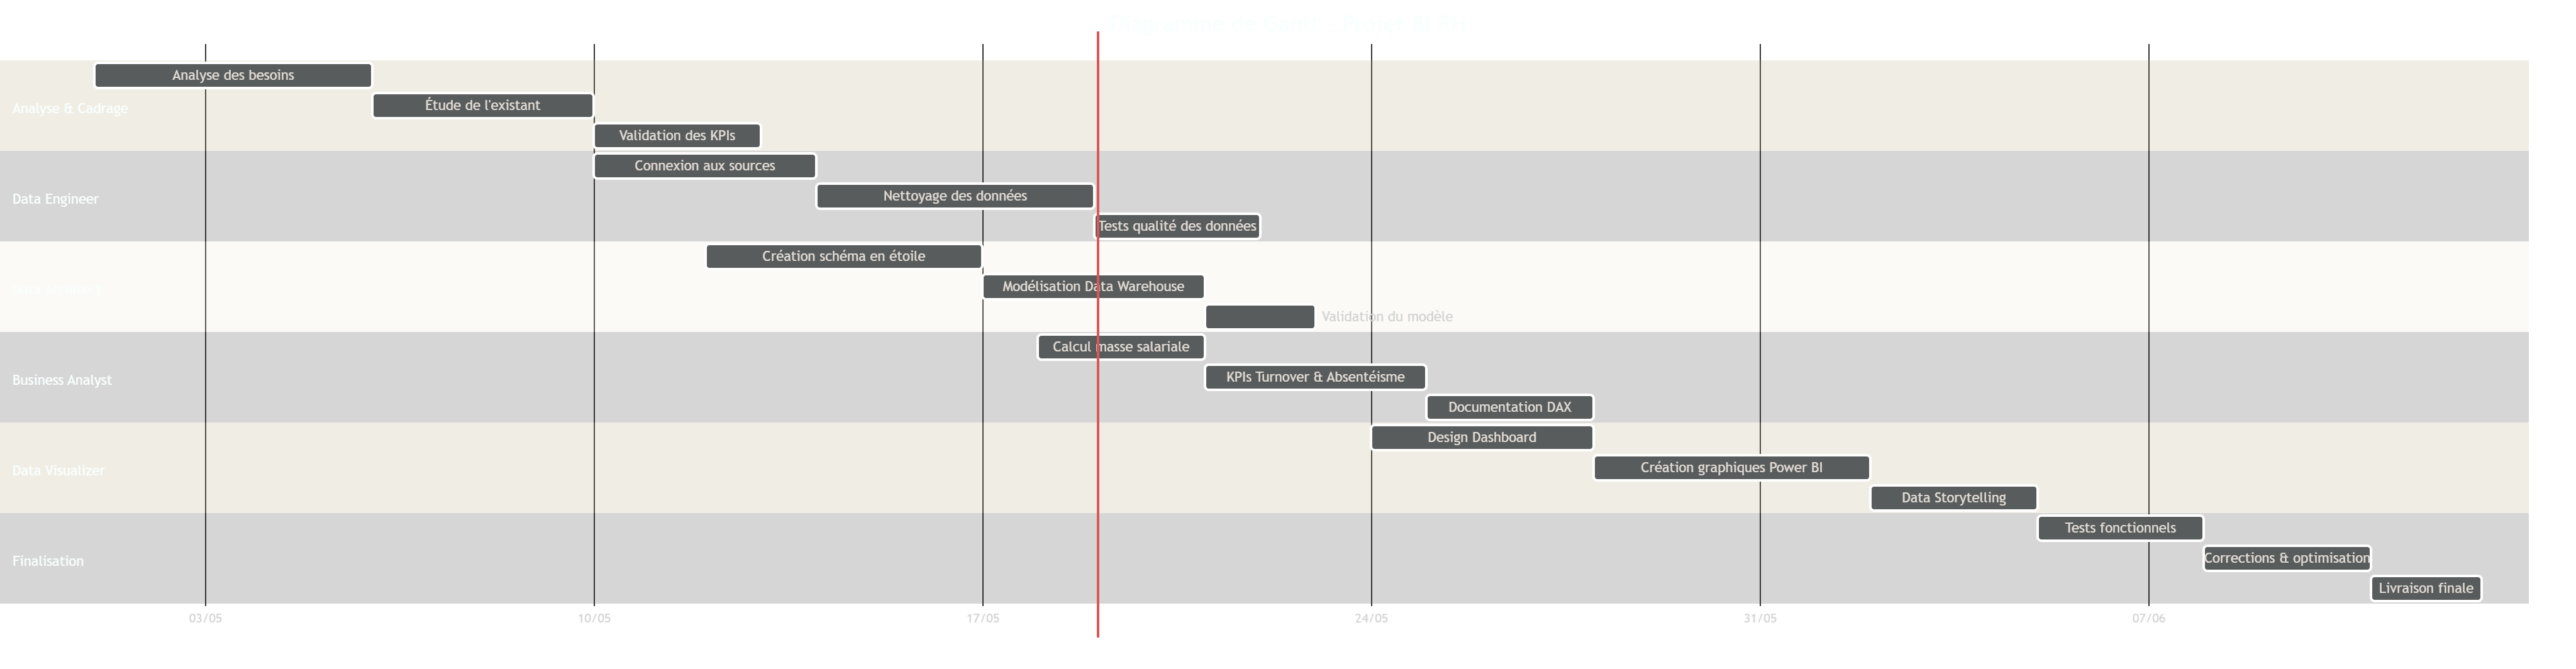
\includegraphics[width=0.8\textwidth]{figures/fig1_2_gantt.png}
    \caption{Diagramme de Gantt du projet}
    \label{fig:gantt}
\end{figure}
